\chapter{前提知識}
\label{chap:prerequisite}
本章では,本研究の前提となる知識に関して説明する.具体的には,代表的な深層生成モデルである変分自己符号化器(Variational Auto-encoder, VAE)とその拡張であるDRAWについてまとめた後,本研究のベースラインとなる生成クエリネットワークについて説明する.

最後に,生成クエリネットワークの確率モデルの考察において用いるメタ学習と呼ばれる機械学習のフレームワークについて説明する.

\section{VAE}
\label{section:VAE}

\begin{figure}[tbp]
\begin{center}
\begin{tikzpicture}
  % Define nodes
  \node[obs] (x) {$\bm{x}$};
  \node[latent, above=of x] (z) {$\bm{z}$};
  \node[const, right=of x] (theta) {$\theta$};

  % Connect the nodes
  \edge {z} {x} ; %
  \edge {theta} {x};
  \edge {theta} {z};
  %\edge [dashed, xsift=-0.1] {x} {z} ;

\end{tikzpicture}
\caption{VAEのグラフィカルモデル}
\label{fig:gm_vae}
\end{center}
\end{figure}

{\bf 変分自己符号化器}({\bf Variational Auto-encoder}, 以下{\bf VAE})\cite{vae}は,深層生成モデルの一種である.
VAEでは,データ$\bm{x} \in \mathbb{R}^n$はある潜在変数$\bm{z} \in \mathbb{R}^m$から生成されると考え,その確率的生成過程$p(\bm{x}|\bm{z})$を多層ニューラルネットワークを用いてモデル化する.
つまり,Fig. \ref{fig:gm_vae}のようなグラフィカルモデルで表現される確率モデルを仮定し,そのパラメータ$\theta$をニューラルネットワークのパラメータとして表現する.
ここでは,Fig. \ref{fig:mnist}のような$28\times28$ピクセルの手書き数字画像データセットMNIST\cite{MNIST}の例を用いて説明する.
データ$\bm{x}$は手書き数字の画像に該当するが,これはそれぞれの要素が1つのピクセルの値に相当する$28\times28=784$次元のベクトルで表された高次元な表現である.
潜在変数$\bm{z}$は,データ$\bm{x}$をより低次元に表現する.
これは,画像のような高次元なデータは画像空間上の非常に限られた領域に局所的に存在しており,それらはより低次元に表現可能であるとする多様体仮説に基づいている.

\begin{figure}[tbp]
\begin{center}
\includegraphics{./figures/mnist.png}
\caption{MNISTデータセットの手書き数字画像}
\label{fig:mnist}
\end{center}
\end{figure}

すると,データの分布$p(\bm{x})$は,$\theta$によってパラメータ化された条件付き分布$p(\bm{x}| \bm{z}; \theta)$を用いて,
\begin{equation}
p(\bm{x}) = \int p(\bm{x}|\bm{z};\theta) p(\bm{z}) d\bm{z} \label{eq:vae}
\end{equation}
と書くことができる.
%ここで,$p(\bm{x}| \bm{z}; \theta)$は潜在変数からデータを生成するため,デコーダと呼ばれる.
VAEでは,潜在変数の分布について,以下の2つの仮定を置く.
\begin{eqnarray}
p(\bm{z}) &=& \mathcal{N}(\bm{z}|0,\bm{I}) \label{eq:z}\\
p(\bm{z}|\bm{x}) &=& \mathcal{N}(\bm{z}|\mu(\bm{x}),\sigma(\bm{x}))	\label{eq:z_cond}
\end{eqnarray}
式(\ref{eq:z})は,潜在空間が標準正規分布に従っているという仮定であり,式(\ref{eq:z_cond})は,$\bm{x}$に条件づけられた潜在変数の分布が正規分布に従うという仮定である.
ベイズ統計では$p(\bm{z})$は事前分布と呼ばれ,データ$\bm{x}$を観測した後の分布$p(\bm{z}|\bm{x})$は事後分布と呼ばれる.
%また,潜在変数を観測データから推定することを,推論(inference)と呼ぶ.
%$p(\bm{z}|\bm{x})$は,データを低次元の潜在空間に埋め込むため,エンコーダと呼ばれる.
$p(\bm{z}|\bm{x})$を解析的に求めることができるケースは非常に限られており,これが解けない場合,近似分布$q(\bm{z}|\bm{x})$を導入して$p(\bm{z}|\bm{x})$を近似することがベイズ統計ではよく行われる.
VAEでも,$p(\bm{z}| \bm{x})$を別のパラメータ$\phi$を用いて$q(\bm{z}|\bm{x};\phi)$によって近似する.
$p(\bm{z}|\bm{x})$はガウス分布を仮定しているため,$q(\bm{z}|\bm{x};\phi)$もガウス分布を仮定する.
VAEでは,この近似分布$q(\bm{z}|\bm{x};\phi)$もニューラルネットワークを用いて表現する.
%VAEはエンコーダとデコーダの両者をニューラルネットワークで定義する.

VAEの目的はデータの分布$p(\bm{x})$を推定することであるため,目的関数は式(\ref{eq:vae})の尤度を最大化することである.
しかし,式(\ref{eq:vae})は$\bm{z}$の周辺化を含み,これを解析的に求めることは困難であるため,尤度そのものを計算することはできない.
%そこで,$\theta$によってパラメータ化されたデコーダ$p(\bm{x}|\bm{z}; \theta)$と,$\phi$によってパラメータ化されたエンコーダ$q(\bm{z}|\bm{x};\phi)$を用いて,式(\ref{eq:vae})の対数をとって,その変分下限を次のように導出する.
そこで,式(\ref{eq:vae})に先ほど定義した$p(\bm{z}|\bm{x})$の近似分布$q(\bm{z}|\bm{x};\phi)$を導入し,その対数をとることで,以下のような変分下限を導出する.
\begin{eqnarray}
\log p(\bm{x}) &=& \log \int p(\bm{x}|\bm{z}; \theta) p(\bm{z}) d\bm{z} \nonumber \\
&=& \log \int q(\bm{z}|\bm{x}; \phi) \frac{p(\bm{x}|\bm{z}; \theta) p(\bm{z})}{q(\bm{z}|\bm{x}; \phi)} d\bm{z} \nonumber \\
&\geq& \int q(\bm{z}|\bm{x}; \phi) \log \frac{p(\bm{x}|\bm{z}; \theta) p(\bm{z})}{q(\bm{z}|\bm{x}; \phi)} d\bm{z} \label{eq:jensen}\\
&=& \int q(\bm{z}|\bm{x}; \phi) \log p(\bm{x}|\bm{z}; \theta) d\bm{z} - \int q(\bm{z}|\bm{x}; \phi) \log \frac{q(\bm{z}|\bm{x}; \phi)}{p(\bm{z})} d\bm{z} \nonumber \\
&=& \mathbb{E}_{\bm{z} \sim q(\bm{z}|\bm{x}; \phi)} [\log p(\bm{x}|\bm{z}; \theta)] - \mathrm{D_{KL}}(q(\bm{z}|\bm{x}; \phi) \| p(\bm{z})) \label{eq:elbo}
\end{eqnarray}
ここで,式(\ref{eq:jensen})でイェンセンの不等式(Jensen's inequality)を用いている.
式(\ref{eq:elbo})の第2項の$\mathrm{D_{KL}}$(カルバックライブラー距離)は,いま$p(\bm{z})$,$q(\bm{z}|\bm{x}; \phi)$共にガウス分布を仮定しているため,解析的に計算することができる.
一方,式(\ref{eq:elbo})の第1項は,解析的には計算できないため,$q(z|x; \phi)$からサンプリングされる$L$個の$\bm{z}$を用いて$\frac{1}{L} \sum_{l} \log p(\bm{x}|\bm{z})$でモンテカルロ近似する.通常,$p(\bm{x}|\bm{z})$はベルヌーイ分布や正規分布とし,その尤度を計算する.
VAEではこの変分下限を目的関数として最大化するように,誤差逆伝播法でニューラルネットワークのパラメータ$\theta$と$\phi$の最適化を行う.
しかし,ここで$q(\bm{z}|\bm{x}; \phi)$からサンプリングを行う部分で勾配の計算ができず,計算グラフが途切れてしまって,誤差逆伝搬法を用いた最適化ができなくなってしまうという問題が生じる.
これを解決するために,VAEでは{\bf 再パラメータ化トリック}({\bf reparameterization trick})を使用する.
%Fig. \ref{fig:reparam}に,再パラメータ化トリックの概略を示す.
通常のサンプリングを行う場合,正規分布$q(\bm{z}|\bm{x}; \phi)$の母数である平均$\mu (\bm{x})$と標準偏差$\sigma (\bm{x})$がニューラルネットワークによって出力された後,$N(\mu (\bm{x}), \sigma (\bm{x}))$から$\bm{z}$をサンプリングするが,これでは計算グラフが途切れてしまう.
そこで,再パラメータ化トリックでは,$\mathcal{N}(\mu (\bm{x}), \sigma (\bm{x}))$から直接サンプリングを行う代わりに,標準正規分布$\mathcal{N}(\bm{0},\bm{I})$からサンプルされる変数$\epsilon$を用いて,$\bm{z}=\mu (\bm{x})+ \epsilon \cdot \sigma (\bm{x})$と計算することによって,計算グラフを途切らせることなく,確率的なサンプリングを可能にする.
以上がVAEの学習の概要である.このように学習されたVAEは,事前分布$p(\bm{z})$から$\bm{z}$をサンプリングし,デコーダを通すことでFig. \ref{fig:vae}のような新たなデータを生成することができる.左は顔画像のデータセットFrey Faceを用いて学習したVAEによって生成された画像,右はMNISTで学習したVAEの生成画像である(ただし,Fig. \ref{fig:mnist}とは白黒が反転していることに注意されたい).

\begin{figure}[tbp]
  \begin{center}
    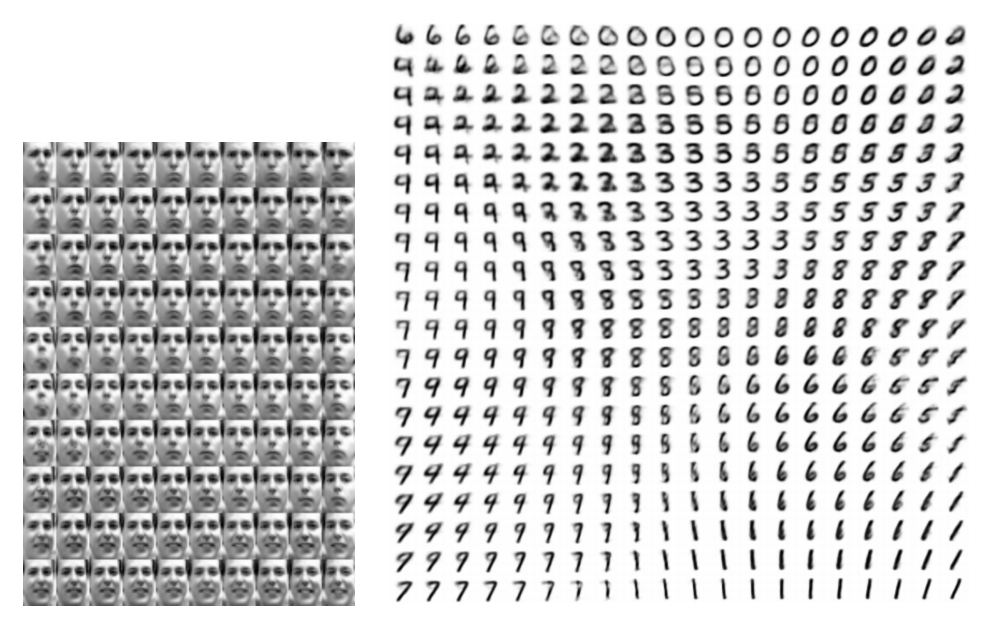
\includegraphics[width=\linewidth]{./figures/vae.png}
    \caption{VAEを用いて生成された画像の例(\cite{vae}より引用)}
    \label{fig:vae}
  \end{center}
\end{figure}

VAEの発展手法として,{\bf 条件付き変分符号化器}({\bf Conditional Variational Auto-encoder}, 以下{\bf CVAE})\cite{Sohn2015}がある.CVAEでは求める分布を$p(\bm{x})$からラベル$y$などで条件付けた分布$p(\bm{x}|\bm{y})$に変更する.例えば,先ほどのMNISTの例を挙げると,手書き数字画像の生成過程を潜在変数$\bm{z}$と1などの数字のラベル($\bm{y}$)を用いてFig. \ref{fig:gm_cvae}のようなグラフィカルモデルで定義することで,1の数字が書かれた手書き数字画像の生成などを可能にするというものである.それに伴い,最適化する目的関数は以下のような条件付き尤度$p(\bm{x}|\bm{y})$の変分下限となり,また事前分布$p(\bm{z}|\bm{y})$もニューラルネットを用いてモデル化する.
\begin{eqnarray}
\log p(\bm{x}|\bm{y}) &=& \log \int p(\bm{x}|\bm{y},\bm{z}; \theta) p(\bm{z}|\bm{y}; \theta) d\bm{z} \nonumber \\
&=& \log \int q(\bm{z}|\bm{x}, \bm{y}; \phi) \frac{p(\bm{x}|\bm{y}, \bm{z}; \theta) p(\bm{z}|\bm{y}; \theta)}{q(\bm{z}|\bm{x}, \bm{y}; \phi)} d\bm{z} \nonumber \\
&\geq& \int q(\bm{z}|\bm{x}, \bm{y}; \phi) \log \frac{p(\bm{x}|\bm{y}, \bm{z}; \theta) p(\bm{z}|\bm{y})}{q(\bm{z}|\bm{x}, \bm{y}; \phi)} d\bm{z} \nonumber \\
&=& \int q(\bm{z}|\bm{x}, \bm{y}; \phi) \log p(\bm{x}|\bm{y}, \bm{z}; \theta) d\bm{z} - \int q(\bm{z}|\bm{x}, \bm{y}; \phi) \log \frac{q(\bm{z}|\bm{x}, \bm{y}; \phi)}{p(\bm{z}|\bm{y})} d\bm{z} \nonumber \\
&=& \mathbb{E}_{\bm{z} \sim q(\bm{z}|\bm{x}, \bm{y}; \phi}) [\log p(\bm{x}|\bm{y}, \bm{z}; \theta)] - \mathrm{D_{KL}}(q(\bm{z}|\bm{x}, \bm{y}; \phi) \| p(\bm{z}|\bm{y})) \label{eq:celbo}
\end{eqnarray}

\begin{figure}[tbp]
\begin{center}
\begin{tikzpicture}
  % Define nodes
  \node[obs] (x) {$\bm{x}$};
  \node[latent, above=of x] (z) {$\bm{z}$};
  \node[obs, right=of x] (y) {$\bm{y}$};
  \node[const, left=of x] (theta) {$\theta$};

  % Connect the nodes
  \edge {z} {x} ; %
  \edge {y} {x};
  \edge {y} {z};
  \edge {theta} {x};
  \edge {theta} {z};
  %\edge [dashed, xsift=-0.1] {x} {z} ;

\end{tikzpicture}
\caption{CVAEのグラフィカルモデル}
\label{fig:gm_cvae}
\end{center}
\end{figure}

このCVAEは,数字のような単純なラベルだけでなく,文章を条件付けとして用いて,その文章に対応するような画像を生成するモデルの研究(Fig. \ref{fig:image_from_caption}参照)\cite{Mansimov2015}など,その応用範囲は多岐に及ぶ\cite{Larsen2015}.

\begin{figure}[tbp]
  \begin{center}
    \includegraphics[width=\linewidth]{./figures/image_from_caption.png}
    \caption{文章から画像を生成するモデルの生成例(\cite{Mansimov2015}より引用)}
    \label{fig:image_from_caption}
  \end{center}
\end{figure}

\section{DRAW}
\label{section:DRAW}
{\bf Deep Recurrent Attentive Writer}(以下{\bf DRAW})\cite{Gregor2015, Gregor2016}はVAEの発展手法の1つである.VAEでは,潜在変数の事前分布を標準正規分布としていたが,これによりモデルの表現力が制限されてしまい,カラー画像などのより複雑なデータの生成過程をモデル化するには不十分となっていた.そこで,DRAWでは,以下のような自己回帰モデルを用いて潜在変数の分布をモデル化する.

\begin{equation}
p(\bm{z}) = \prod_{l=1}^{L}p_{l}(\bm{z_{l}}|\bm{z_{<l}}) \label{eq:pdraw}
\end{equation}

これに伴い,データ$\bm{x}$から潜在変数$\bm{z}$への推論分布も以下のように自己回帰モデルを用いて行われる.

\begin{equation}
q ( \bm{z} | \bm{x} ) = \prod _ { l = 1 } ^ { L } q _ { l }( \bm{z _ { l } } | \bm{x} , \bm{z _ { < l }}) \label{eq:qdraw}
\end{equation}

ただし,$p_l(\bm{z_l}|\bm{z_{<l}})$と$q_l(\bm{z_l}|\bm{x}, \bm{z_{<l}})$はそれぞれ正規分布に従うと仮定する.
このようにモデル化することで,$p(\bm{z})$と$q ( \bm{z} | \bm{x} )$は,より複雑な分布を表現することができるようになり,単純な正規分布のみで潜在変数を表現するVAEと比較して,多様なデータの生成過程を表現可能となる.

これを踏まえると,DRAWで仮定するデータの生成過程はFig. \ref{fig:gm_draw}のようなグラフィカルモデルで表現することができる.ただし,簡単のため,DRAWのように自己回帰モデルを含むような生成モデルのグラフィカルモデルを今後はFig. \ref{fig:gm_draw_simple}のように簡潔化して表記することとする.

\begin{figure}[tbp]
\begin{center}
\begin{tabular}{c}
\begin{minipage}{0.5\linewidth}
\begin{center}
\begin{tikzpicture}
  % Define nodes
  \node[obs] (x) {$\bm{x}$};
  \node[latent, above=of x] (z_2) {$\bm{z_2}$};
  \node[latent, left=of z_2] (z_1) {$\bm{z_1}$};
  \node[latent, right=of z_2] (z_L) {$\bm{z_L}$};
  \node [const, right=of x] (theta) {$\theta$};

  % Connect the nodes
  \edge {z_1} {x} ; %
  \edge {z_2} {x} ; %
  \edge {z_L} {x} ; %
  
  \edge {z_1} {z_2} ; %
  \edge [bend left] {z_1} {z_L} ; %
  \edge [bend left] {z_2} {z_L} ; %
  \edge [-, loosely dotted, very thick] {z_2} {z_L};
  \edge {theta} {z_1};
  \edge {theta} {z_2};
  \edge {theta} {z_L};
  \edge {theta} {x};
  
  % Plates
  \plate {z} {(z_1)(z_2)(z_L)} {$\bm{z}$} ;
  %\plate {} {(w)(y)(yx.north west)(yx.south west)} {$M$} ;

\end{tikzpicture}
\end{center}
\caption{DRAWのグラフィカルモデル}
\label{fig:gm_draw}
\end{minipage}

\begin{minipage}{0.5\linewidth}
\begin{center}
\begin{tikzpicture}
  % Define nodes
  \node[obs] (x) {$\bm{x}$};
  \node[latent, above=of x] (z) {$\bm{z}$};
  \node[const, right=of x] (theta) {$\theta$};
 
  % Connect the nodes
  \edge {z} {x} ; %
  \edge [loop above] {z} {z} ; %
  \edge {theta} {z};
  \edge {theta} {x};
     
  % Plates
  %\plate {} {(w)(y)(yx.north west)(yx.south west)} {$M$} ;

\end{tikzpicture}
\end{center}
\caption{DRAWのグラフィカルモデル(簡易版)}
\label{fig:gm_draw_simple}
\end{minipage}
\end{tabular}
\end{center}
\end{figure}

DRAWはVAEと同様に対数尤度$ \log p(\bm{x})$の変分下限を最大化によって学習されるが,潜在変数の分布が複数の分布の積によって表されるため,第二項が以下のようにそれぞれの分布間のカルバックライバー距離の和となる.

\begin{eqnarray}
{ \mathrm { D_{KL} } } ( q ( \bm{z} | \bm{x} ) | | p ( \bm{z} ) )
&=& \mathrm{ D_{KL} }( \prod _ { l = 1 } ^ { L } q _ { l } (\bm{ z _ { l }} | \bm{x} , \bm{z _ { < l }} ) \| \prod _ { l = 1 } ^ { L } p _ { l } (\bm{ z _ { l }} | \bm{z _ { < l }} ) ) \nonumber \\
&=& \sum _ { l = 1 } ^ { L } \mathbb { E } _ { q ( \bm{ z  _ { < l }} | \bm{x} ) } [ \mathrm { D } _ { \mathrm { KL } } ( q _ { l } ( \bm{z _ { l }} | \bm{x} , \bm{z _ { < l }} ) | | p _ { l } ( \bm{z _ { l }} | \bm{z _ { < l }} ) ) ] \nonumber \\
&=& \mathbb { E } _ { q(\bm{ z } | \bm{x}) } [\sum _ { l = 1 } ^ { L } \mathrm { D } _ { \mathrm { KL } } ( q _ { l } ( \bm{z _ { l }} | \bm{x} , \bm{z _ { < l }} ) | | p _ { l } ( \bm{z _ { l }} | \bm{z _ { < l }} ) ) ]
\end{eqnarray}

よって,DRAWでは以下の変分下限を最大化することで学習される.
\begin{eqnarray}
\log p(\bm{x}) 
&\geq& \mathbb{E}_{\bm{z} \sim q(\bm{z}|\bm{x}; \phi}) [\log p(\bm{x}|\bm{z}; \theta)] - \sum _ { l = 1 } ^ { L } \mathrm { E } _ { q ( \mathrm { z } _ { < l } | x ) } [ \mathrm { D } _ { \mathrm { KL } } ( q _ { l } ( z _ { l } | x , z _ { < l } ) | | p _ { l } ( z _ { l } | z _ { < l } ) ) ] \nonumber \\
&=& \mathbb{E}_{\bm{z} \sim q(\bm{z}|\bm{x}}) [\log p(\bm{x}|\bm{z}) - \sum _ { l = 1 } ^ { L } \mathrm { D } _ { \mathrm { KL } } ( q _ { l } ( z _ { l } | x , z _ { < l } ) | | p _ { l } ( z _ { l } | z _ { < l } ) ) ] \label{eq:drawelbo}
\end{eqnarray}

DRAWで学習されたモデルは,その表現力の高さから,Fig. \ref{fig:draw_example}のようにカラー画像でも鮮明な画像を生成することができる.

\begin{figure}[tbp]
  \begin{center}
    \includegraphics[width=0.5\linewidth]{./figures/draw_example.png}
    \caption{SVHNデータセットで学習したDRAWの生成画像例(\cite{Gregor2015}より引用)}
    \label{fig:draw_example}
  \end{center}
\end{figure}

\section{生成クエリネットワーク}

\begin{figure}[tbp]
  \begin{center}
    \includegraphics[width=\linewidth]{./figures/gqn_flow.png}
    \caption{生成クエリネットワークの学習の流れ}
    \label{fig:gqn_flow}
  \end{center}
\end{figure}

ここからは本研究のベースラインとなる生成クエリネットワークについて説明する.生成クエリネットワークも深層生成モデルの一種であり,その学習法はCVAEやDRAWをベースとしている.生成クエリネットワークは,3次元空間上のある視点からの観測画像がいくつか与えられた状況において,別の視点からの観測画像を予測して生成するモデルである.生成クエリネットワークの学習の流れをFig. \ref{fig:gqn_flow}に示す.生成クエリネットワークの学習に用いるデータセットは,3次元環境での様々な視点からの観測画像からなり,それぞれの環境は異なる物体で構成されている.それぞれの環境のことをここでは{\bf シーン}と呼ぶ.学習時には,まず多数あるシーンの中からランダムに1つを選択し,選択したシーン$i$の中から,モデルが事前に知ることのできる観測画像をいくつか選択する.この事前に与えられた観測画像とその視点座標のペア群($\bm{x_i^{1..M}}, \bm{v_i^{1..M}}$)をここでは{\bf コンテキスト}と呼ぶ.そして,モデルはそのコンテキストを元に未知の別の視点($\bm{v_i^q}$, ここではクエリと呼ぶ)からの観測画像$\bm{x_i^q}$を予測して生成し,正しい予測が行えるように学習を行う.つまり,生成クエリネットワークでは,条件付き尤度$p(\bm{x^q} | \bm{v^q}, \bm{x^{1..M}}, \bm{v^{1..M}} ; \theta)$を最大化するように学習を行う.そこで,VAEやDRAWと同様に,潜在変数$\bm{z_i}$を導入して,最大化したい条件付き尤度の変分下限を以下のように導く.ただし,ここでは簡単のため,シーンを表す表記$i$を省略する.

\begin{eqnarray}
&\log& p(\bm{x^q} | \bm{v^q}, \bm{x^{1..M}}, \bm{v^{1..M}} ; \theta) \nonumber \\
&=& \log \int p(\bm{x^q} | \bm{v^q}, \bm{x^{1..M}}, \bm{v^{1..M}}, \bm{z}; \theta) p(\bm{z^q} | \bm{v^q}, \bm{x^{1..M}}, \bm{v^{1..M}}; \theta) d\bm{z} \nonumber \\
&=& \log \int q(\bm{z} | \bm{x^q}, \bm{v^q}, \bm{x^{1..M}}, \bm{v^{1..M}} ; \phi )
	\frac{p(\bm{x^q} | \bm{v^q}, \bm{x^{1..M}}, \bm{v^{1..M}}, \bm{z}; \theta) \pi(\bm{z} | \bm{v^q}, \bm{x^{1..M}}, \bm{v^{1..M}}; \theta)}
{q(\bm{z} | \bm{x^q}, \bm{v^q}, \bm{x^{1..M}}, \bm{v^{1..M}} ; \phi )} d\bm{z} \nonumber \\
&\geq&  \int q(\bm{z} | \bm{x^q}, \bm{v^q}, \bm{x^{1..M}}, \bm{v^{1..M}} ; \phi )
	\log \frac{p(\bm{x^q} | \bm{v^q}, \bm{x^{1..M}}, \bm{v^{1..M}}, \bm{z}; \theta) \pi(\bm{z} | \bm{v^q}, \bm{x^{1..M}}, \bm{v^{1..M}}; \theta)}
{q(\bm{z} | \bm{x^q}, \bm{v^q}, \bm{x^{1..M}}, \bm{v^{1..M}} ; \phi )} d\bm{z} \nonumber \\
&=& \int q(\bm{z} | \bm{x^q}, \bm{v^q}, \bm{x^{1..M}}, \bm{v^{1..M}} ; \phi )
\log p(\bm{x^q} | \bm{v^q}, \bm{x^{1..M}}, \bm{v^{1..M}}, \bm{z}; \theta) d\bm{z} \nonumber \\
	&\quad& - \int q(\bm{z} | \bm{x^q}, \bm{v^q}, \bm{x^{1..M}}, \bm{v^{1..M}} ; \phi )
		\log \frac {q(\bm{z} | \bm{x^q}, \bm{v^q}, \bm{x^{1..M}}, \bm{v^{1..M}} ; \phi )}
	{\pi(\bm{z} | \bm{v^q}, \bm{x^{1..M}}, \bm{v^{1..M}}; \theta)} d\bm{z} \nonumber \\
&=& \mathbb{E}_{\bm{z} \sim q(\bm{z} | \bm{x^q}, \bm{v^q}, \bm{x^{1..M}}, \bm{v^{1..M}} ; \phi )}
	[\log p(\bm{x^q} | \bm{v^q}, \bm{x^{1..M}}, \bm{v^{1..M}}, \bm{z}; \theta) ]
	- \mathrm { D } _ { \mathrm { KL } }(q||\pi) \label{eq:gqn_elbo}
\end{eqnarray}

さらに,生成クエリネットワークでは,DRAWと同様に潜在変数$\bm{z}$を自己回帰モデルで表現しているため,最適化する変分下限は以下のようになる.
\begin{equation}
\mathbb{E}_{\bm{z} \sim q(\bm{z} | \bm{x^q}, \bm{v^q}, \bm{x^{1..M}}, \bm{v^{1..M}} ; \phi )}
[\log p(\bm{x^q} | \bm{v^q}, \bm{x^{1..M}}, \bm{v^{1..M}}, \bm{z}; \theta)
- \sum _ { l = 1 } ^ { L } {\mathrm { D } _ { \mathrm { KL } }}
	(q_l || \pi_l)] \label{eq:gqn_draw_elbo}
\end{equation}

$p(\bm{x^q} | \bm{v^q}, \bm{x^{1..M}}, \bm{v^{1..M}}, \bm{z^q}; \theta)$,$q(\bm{z^q} | \bm{x^q}, \bm{v^q}, \bm{x^{1..M}}, \bm{v^{1..M}} ; \phi )$,$\pi(\bm{z} | \bm{v^q}, \bm{x^{1..M}}, \bm{v^{1..M}}; \theta)$はそれぞれニューラルネットワークを用いてモデル化されるが,その際にコンテキスト$\bm{x^{1..M}}, \bm{v^{1..M}}$を入力として,それらを圧縮した変数$\bm{r}$を出力する{\bf 表現ネットワーク}({\bf representation network})を用意しており.この変数$\bm{r}$を元論文内では{\bf シーン表現}と呼んでいる.これは,表現ネットワークがコンテキストに含まれる情報からシーン全体を表すような表現を抽出するように学習されることを意味する.
生成クエリネットワークで仮定するデータの生成過程は,シーン表現$\bm{r}$を考慮すると,Fig. \ref{fig:gm_gqn}のようなグラフィカルモデルで表される.

\begin{figure}[tbp]
\begin{center}
\begin{tikzpicture}
  % Define nodes
  \node[obs] (x_q) {$\bm{x_i^q}$};
  \node[obs, right=of x_q] (v_q) {$\bm{v_i^q}$};
  \node[latent, above=of v_q] (z) {$\bm{z_i}$};
  \node[latent, left=of x_q] (r) {$\bm{r_i}$};
   
   \node[obs, left=of r] (x_k) {$\bm{x_i^k}$};
   \node[obs, left=of x_k] (v_k) {$\bm{v_i^k}$};
   
   % Plates
  \plate {query} {(x_q)(v_q)} {クエリ} ;
  \plate {context} {(x_k)(v_k)} {$k=1,...,M$} ;
  \plate {scene} {(query)(context)(r)(z)} {シーン$i$} ;
   
   \node[const, above=of scene] (theta) {$\theta$};

  % Connect the nodes
  \edge {z} {x} ; %
  
  \edge [loop above] {z} {z} ; %
  
  \edge {v_q} {x_q};
  \edge {v_q} {z};
  
  \edge [dashed] {x_k} {r}
  \edge [bend left, dashed] {v_k} {r}
  
  \edge {r} {x_q};
  \edge {r} {z};
  
  \edge {theta} {z}
  \edge {theta} {x_q}

\end{tikzpicture}
\caption{生成クエリネットワークのグラフィカルモデル}
\label{fig:gm_gqn}
\end{center}
\end{figure}

\section{メタ学習}
\label{section:meta_learning}
ここでは,生成クエリネットワークについて理論的な考察を行う上で用いる{\bf メタ学習}と呼ばれる機械学習のフレームワークについて説明する.
メタ学習とは,複数のデータセットが与えられ,それぞれのデータセットごとにドメインやタスクが異なるような状況において,学習対象のドメインやタスクに応じて学習器のバイアスを決定するためのメタ知識を獲得する枠組みを指す\cite{Vilalta2002}.画像認識の場合の簡単な例をあげると,学習器には様々なソースから手に入れた画像データセットが与えられるとする.しかし,あるデータセットは実世界で撮られた写真で構成されているのに対し,別のデータセットはイラスト画像で構成されている,といったように,データセットごとに画像の性質は様々である.このとき,学習器は出力すべき「犬」や「車」といったラベルは共通である,つまり{\bf タスク}は共通であるのに対し,入力となる画像が従う確率空間(これを{\bf ドメイン}と呼ぶ)はデータセット間で明らかに異なる.このような場合に,メタ学習では写真やイラストというドメインに固有な知識とドメイン間で共通の知識({\bf メタ知識})を分けて学習することによって,未知のドメインに対してもメタ知識を用いて少ないデータからドメイン固有の知識を獲得し,正しく分類を行えるようにモデルのバイアスを決定する.ここでは,タスクが共通でドメインが異なるような場合の例を挙げたが,ドメインが共通でタスクが異なるような場合も同様のアプローチでメタ学習の枠組みを用いることができる.

\begin{figure}[tbp]
  \begin{center}
    \includegraphics[width=\linewidth]{./figures/meta_learning.png}
    \caption{メタ学習におけるデータセットの典型例(\cite{Ravi2016}より引用)}
    \label{fig:ml_example}
  \end{center}
\end{figure}

メタ学習の手法は様々なものが提案されているが\cite{maml, Ravi2016},\cite{Gordon2018}では多くのメタ学習手法を統一的に定式化するフレームワーク({\bf ML-PIP})を提案している.
ML-PIPでは,メタ学習を行う対象となる複数のデータセットのデータ群の生成過程をFig. \ref{fig:ml_pip}のようにモデリングする.
$\theta$は全てのデータセットで共有のメタ知識をもつパラメータであり,$\psi^{(t)}$は$t$番目のデータセットに固有の知識をもつパラメータ(もしくは変数)である.

\begin{figure}[tbp]
\begin{center}
\begin{tikzpicture}
  % Define nodes
  \node[obs] (y) {$\bm{y^{(t)}}$};
  \node[obs, left=of y] (x) {$\bm{x^{(t)}}$};
  \node[latent, right=of y] (psi) {$\psi^{(t)}$};
   
   \node[obs, right=of psi] (y_tilde) {$\bm{\tilde{y}^{(t)}}$};
   \node[obs, right=of y_tilde] (x_tilde) {$\bm{\tilde{x}^{(t)}}$};
   
   \node[const, above=of psi] (theta) {$\theta$};

  % Connect the nodes  
  \edge {x} {y}
  \edge {x_tilde} {y_tilde};
  \edge {psi} {y_tilde};
  \edge {psi} {y};
  
  \edge {theta} {y};
  \edge {theta} {y_tilde};
  \edge {theta} {psi};

  % Plates
  \plate {test} {(x_tilde)(y_tilde)} {テストデータセット} ;
  \plate {train} {(x)(y)} {訓練データセット$D^{(t)}$} ;
  \plate {} {(train)(test)(psi)} {$t$番目のデータセット} ;

\end{tikzpicture}
\caption{ML-PIPのグラフィカルモデル}
\label{fig:ml_pip}
\end{center}
\end{figure}

メタ学習の目的は,未知のデータセットが与えられた状況において,少ない訓練データ$D ^ { ( t ) } = \{ ( x _ { n } ^ { ( t ) } , y _ { n } ^ { ( t ) } ) \} _ { n = 1 } ^ { N _ { t } }$からそのデータセット固有の知識を獲得して,テストデータに対して正しい予測を行うことであるから,メタ学習の訓練時には,複数のデータセットを活用して,条件付き尤度$\sum_{t} p(\bm{\tilde{y}^{(t)}} | \bm{\tilde{x}^{(t)}}, D^{(t)}; \theta)$を最大化することを目的関数として学習する.すると,$t$番目のデータセットにおいて,$p(\bm{\tilde{y}^{(t)}} | \bm{\tilde{x}^{(t)}}, D^{(t)}; \theta)$は$\theta$と$\psi$を用いて以下のように表される.

\begin{equation}
p \left( \bm{\tilde { y } ^ { ( t ) }} | \bm{\tilde { x } ^ { ( t ) }}, D^{(t)} ; \theta \right) = \int p \left( \bm{\tilde { y } ^ { ( t ) }} | \bm{\tilde { x } ^ { ( t ) }} , \psi ^ { ( t ) } ; \theta \right) p \left( \psi ^ { ( t ) } | D^{(t)} ; \theta \right) \mathrm { d } \psi ^ { ( t ) } \label{eq:meta_likelihood}
\end{equation}

この尤度を最大化するようにパラメータ$\theta$を最適化することで,真の分布に近い$p(\bm{\tilde{y}^{(t)}} | \bm{\tilde{x}^{(t)}}, D^{(t)};\theta)$を得ることができるが,ここで問題となるのが,$p ( \psi ^ { ( t ) } | D^{(t)}; \theta)$は一般に解析的に求めるのが困難であるという点である.そこで新たなパラメータ$\phi$を用いて,$q(\psi ^ { ( t ) } | D^{(t)}; \phi )$を作り,これで$p ( \psi ^ { ( t ) } | D^{(t)}; \theta )$を近似する.このようにある変数の分布を事後分布で近似推論することを一般に{\bf amortized inference}と呼ばれている.$\psi$の分布をこのように近似すると,式(\ref{eq:meta_likelihood})は以下のように近似される.

\begin{equation}
q ( \bm{\tilde { y } ^ { ( t ) }} | \bm{\tilde { x } ^ { ( t ) }} , D^{(t)}; \theta , \phi ) = \int p ( \bm{\tilde { y } ^ { ( t ) }} | \bm{\tilde { x } ^ { ( t ) }} , \psi ^ {(t)} ; \theta ) q ( \psi ^ { ( t ) } | D ^ { ( t ) } ; \phi ) \mathrm { d } \psi ^ { ( t ) } \label{eq:meta_approximation}
\end{equation}

ここでの目的は$q ( \bm{\tilde { y } ^ { ( t ) }} | \bm{\tilde { x } ^ { ( t ) }} , D^{(t)}; \theta , \phi )$が真の分布$p ( \bm{\tilde { y } ^ { ( t ) }} | \bm{\tilde { x } ^ { ( t ) }} ,D^{(t)})$に近づくように$\theta$と$\phi$を学習することであるから,以下のように定式化される.
\begin{equation}
\hat{\theta}, \hat{\phi} = \argmin _ { \theta, \phi } \mathrm{D_{KL}} [p ( \bm{\tilde { y } ^ { ( t ) }} | \bm{\tilde { x } ^ { ( t ) }} ; \theta^{\ast} ) || q ( \bm{\tilde { y } ^ { ( t ) }} | \bm{\tilde { x } ^ { ( t ) }} ; \theta , \phi ) ]  = \argmax _ {\theta, \phi } q ( \bm{\tilde { y } ^ { ( t ) }} | \bm{\tilde { x } ^ { ( t ) }} ; \theta , \phi )
\end{equation}

よって,式(\ref{eq:meta_approximation})を最大化するように学習を行えば良い.これが,ML-PIPによるメタ学習の定式化である.

メタ学習の手法の違いは,主に$q ( \bm{\tilde { y } ^ { ( t ) }} | \bm{\tilde { x } ^ { ( t ) }} , D^{(t)}; \theta , \phi )$の設計による.\cite{maml}では,$\psi$をニューラルネットワークのパラメータの初期値として定義し,それを勾配法を用いて最適化するのに対し,\cite{CNP, NP}では$q ( \bm{\tilde { y } ^ { ( t ) }} | \bm{\tilde { x } ^ { ( t ) }} , D^{(t)}; \theta , \phi )$を変数$\psi$を出力するニューラルネットワークとして定義している.